\documentclass[12pt,]{article}
\usepackage{lmodern}
\usepackage{amssymb,amsmath}
\usepackage{ifxetex,ifluatex}
\usepackage{fixltx2e} % provides \textsubscript
\ifnum 0\ifxetex 1\fi\ifluatex 1\fi=0 % if pdftex
  \usepackage[T1]{fontenc}
  \usepackage[utf8]{inputenc}
\else % if luatex or xelatex
  \ifxetex
    \usepackage{mathspec}
  \else
    \usepackage{fontspec}
  \fi
  \defaultfontfeatures{Ligatures=TeX,Scale=MatchLowercase}
    \setmainfont[]{Times New Roman}
\fi
% use upquote if available, for straight quotes in verbatim environments
\IfFileExists{upquote.sty}{\usepackage{upquote}}{}
% use microtype if available
\IfFileExists{microtype.sty}{%
\usepackage{microtype}
\UseMicrotypeSet[protrusion]{basicmath} % disable protrusion for tt fonts
}{}
\usepackage[margin=2.54cm]{geometry}
\usepackage{hyperref}
\hypersetup{unicode=true,
            pdftitle={Chemical Effects on Mammals},
            pdfauthor={Caroline Reents},
            pdfborder={0 0 0},
            breaklinks=true}
\urlstyle{same}  % don't use monospace font for urls
\usepackage{color}
\usepackage{fancyvrb}
\newcommand{\VerbBar}{|}
\newcommand{\VERB}{\Verb[commandchars=\\\{\}]}
\DefineVerbatimEnvironment{Highlighting}{Verbatim}{commandchars=\\\{\}}
% Add ',fontsize=\small' for more characters per line
\usepackage{framed}
\definecolor{shadecolor}{RGB}{248,248,248}
\newenvironment{Shaded}{\begin{snugshade}}{\end{snugshade}}
\newcommand{\KeywordTok}[1]{\textcolor[rgb]{0.13,0.29,0.53}{\textbf{#1}}}
\newcommand{\DataTypeTok}[1]{\textcolor[rgb]{0.13,0.29,0.53}{#1}}
\newcommand{\DecValTok}[1]{\textcolor[rgb]{0.00,0.00,0.81}{#1}}
\newcommand{\BaseNTok}[1]{\textcolor[rgb]{0.00,0.00,0.81}{#1}}
\newcommand{\FloatTok}[1]{\textcolor[rgb]{0.00,0.00,0.81}{#1}}
\newcommand{\ConstantTok}[1]{\textcolor[rgb]{0.00,0.00,0.00}{#1}}
\newcommand{\CharTok}[1]{\textcolor[rgb]{0.31,0.60,0.02}{#1}}
\newcommand{\SpecialCharTok}[1]{\textcolor[rgb]{0.00,0.00,0.00}{#1}}
\newcommand{\StringTok}[1]{\textcolor[rgb]{0.31,0.60,0.02}{#1}}
\newcommand{\VerbatimStringTok}[1]{\textcolor[rgb]{0.31,0.60,0.02}{#1}}
\newcommand{\SpecialStringTok}[1]{\textcolor[rgb]{0.31,0.60,0.02}{#1}}
\newcommand{\ImportTok}[1]{#1}
\newcommand{\CommentTok}[1]{\textcolor[rgb]{0.56,0.35,0.01}{\textit{#1}}}
\newcommand{\DocumentationTok}[1]{\textcolor[rgb]{0.56,0.35,0.01}{\textbf{\textit{#1}}}}
\newcommand{\AnnotationTok}[1]{\textcolor[rgb]{0.56,0.35,0.01}{\textbf{\textit{#1}}}}
\newcommand{\CommentVarTok}[1]{\textcolor[rgb]{0.56,0.35,0.01}{\textbf{\textit{#1}}}}
\newcommand{\OtherTok}[1]{\textcolor[rgb]{0.56,0.35,0.01}{#1}}
\newcommand{\FunctionTok}[1]{\textcolor[rgb]{0.00,0.00,0.00}{#1}}
\newcommand{\VariableTok}[1]{\textcolor[rgb]{0.00,0.00,0.00}{#1}}
\newcommand{\ControlFlowTok}[1]{\textcolor[rgb]{0.13,0.29,0.53}{\textbf{#1}}}
\newcommand{\OperatorTok}[1]{\textcolor[rgb]{0.81,0.36,0.00}{\textbf{#1}}}
\newcommand{\BuiltInTok}[1]{#1}
\newcommand{\ExtensionTok}[1]{#1}
\newcommand{\PreprocessorTok}[1]{\textcolor[rgb]{0.56,0.35,0.01}{\textit{#1}}}
\newcommand{\AttributeTok}[1]{\textcolor[rgb]{0.77,0.63,0.00}{#1}}
\newcommand{\RegionMarkerTok}[1]{#1}
\newcommand{\InformationTok}[1]{\textcolor[rgb]{0.56,0.35,0.01}{\textbf{\textit{#1}}}}
\newcommand{\WarningTok}[1]{\textcolor[rgb]{0.56,0.35,0.01}{\textbf{\textit{#1}}}}
\newcommand{\AlertTok}[1]{\textcolor[rgb]{0.94,0.16,0.16}{#1}}
\newcommand{\ErrorTok}[1]{\textcolor[rgb]{0.64,0.00,0.00}{\textbf{#1}}}
\newcommand{\NormalTok}[1]{#1}
\usepackage{graphicx,grffile}
\makeatletter
\def\maxwidth{\ifdim\Gin@nat@width>\linewidth\linewidth\else\Gin@nat@width\fi}
\def\maxheight{\ifdim\Gin@nat@height>\textheight\textheight\else\Gin@nat@height\fi}
\makeatother
% Scale images if necessary, so that they will not overflow the page
% margins by default, and it is still possible to overwrite the defaults
% using explicit options in \includegraphics[width, height, ...]{}
\setkeys{Gin}{width=\maxwidth,height=\maxheight,keepaspectratio}
\IfFileExists{parskip.sty}{%
\usepackage{parskip}
}{% else
\setlength{\parindent}{0pt}
\setlength{\parskip}{6pt plus 2pt minus 1pt}
}
\setlength{\emergencystretch}{3em}  % prevent overfull lines
\providecommand{\tightlist}{%
  \setlength{\itemsep}{0pt}\setlength{\parskip}{0pt}}
\setcounter{secnumdepth}{5}
% Redefines (sub)paragraphs to behave more like sections
\ifx\paragraph\undefined\else
\let\oldparagraph\paragraph
\renewcommand{\paragraph}[1]{\oldparagraph{#1}\mbox{}}
\fi
\ifx\subparagraph\undefined\else
\let\oldsubparagraph\subparagraph
\renewcommand{\subparagraph}[1]{\oldsubparagraph{#1}\mbox{}}
\fi

%%% Use protect on footnotes to avoid problems with footnotes in titles
\let\rmarkdownfootnote\footnote%
\def\footnote{\protect\rmarkdownfootnote}

%%% Change title format to be more compact
\usepackage{titling}

% Create subtitle command for use in maketitle
\newcommand{\subtitle}[1]{
  \posttitle{
    \begin{center}\large#1\end{center}
    }
}

\setlength{\droptitle}{-2em}

  \title{Chemical Effects on Mammals}
    \pretitle{\vspace{\droptitle}\centering\huge}
  \posttitle{\par}
  \subtitle{\url{https://github.com/c-reents/DataAnalyticsProject}}
  \author{Caroline Reents}
    \preauthor{\centering\large\emph}
  \postauthor{\par}
    \date{}
    \predate{}\postdate{}
  
\usepackage{booktabs}
\usepackage{longtable}
\usepackage{array}
\usepackage{multirow}
\usepackage{wrapfig}
\usepackage{float}
\usepackage{colortbl}
\usepackage{pdflscape}
\usepackage{tabu}
\usepackage{threeparttable}
\usepackage{threeparttablex}
\usepackage[normalem]{ulem}
\usepackage{makecell}
\usepackage{xcolor}

\begin{document}
\maketitle
\begin{abstract}
Experimental overview. This section should be no longer than 250 words.
\end{abstract}

\newpage

\tableofcontents  \newpage
\listoftables  \newpage
\listoffigures  \newpage

\textless{}Note: set up autoreferencing for figures and tables in your
document\textgreater{}

\begin{verbatim}
## [1] "/Users/carolinereents/Desktop/Data Analytics/EnvironmentalDataAnalytics/FinalProject"
\end{verbatim}

\begin{verbatim}
## -- Attaching packages ------------------------------------------------------------------------ tidyverse 1.2.1 --
\end{verbatim}

\begin{verbatim}
## v ggplot2 3.1.0     v purrr   0.2.5
## v tibble  1.4.2     v dplyr   0.7.8
## v tidyr   0.8.2     v stringr 1.3.1
## v readr   1.1.1     v forcats 0.3.0
\end{verbatim}

\begin{verbatim}
## -- Conflicts --------------------------------------------------------------------------- tidyverse_conflicts() --
## x dplyr::filter() masks stats::filter()
## x dplyr::lag()    masks stats::lag()
\end{verbatim}

\begin{verbatim}
## Loading required package: viridisLite
\end{verbatim}

\begin{verbatim}
## Warning: package 'kableExtra' was built under R version 3.5.2
\end{verbatim}

\section{Research Question and
Rationale}\label{research-question-and-rationale}

This data set includes the effects of certain pharmaceutical or health
care drugs or chemicals on the mortality of various mammals. Each data
point is related to a specific study done on that chemical with a
certain mammal. Mortality is measured in various ``endpoints'' which
refer to how much mortality was seen in each study. There are 24
different chemicals in this data set, large groups of these chemicals
are either cancer-combating drugs or antibiotics. For this project I aim
to determine if different mammals are more suscepitble to death from
being exposed to these chemicals, or if mortality is highly dependent on
concentration of chemical. I also want to determine if the cancer drugs
and the antibiotics differ in their likelihood to cause death.

\newpage

\section{Dataset Information}\label{dataset-information}

The following is a list of all chemicals tested in this data set pulled
from the ECOTOX webpage. Each data point is the result of a study, so
each data point seen on visualizations represents the findings of one or
a group of researchers published study.

The data was pulled filtering for mammals, effects of mortality, all
endpoints, and chemical subgroup ``pharmaceutical personal care
products''. The drugs tested in this data set were:

\begin{itemize}
\tightlist
\item
  17alpha-ethynylestradiol : used in BC
\item
  6-mercaptopurine : used for cancer and autoimmune
\item
  Ampicillin - antibiotic
\item
  Betamethasone - steroid
\item
  Clindamyacin - antibiotic
\item
  Dexamethasone - steroid
\item
  Dexamethasone sodium - steroid
\item
  Diazepam - pain killer
\item
  Dimenhydrinate - motion sickness
\item
  Erythomycin - antibiotic
\item
  Gentamycin - antibiotic
\item
  Lindane - treats scabies
\item
  Methimazole - treats hyperthyroid
\item
  Methotrexate - cancer autoimmune treatment
\item
  Metronidazole - antibiotic
\item
  Phenobarbital - sedative
\item
  Prednisone - steroid
\item
  Propranolol - beta-blocker
\item
  Tetracycline - antibiotic
\item
  Tetracycline hydrochloride - antibiotic
\item
  Thalidomide - cancer treeatment
\item
  Trans-Retinoic acid - cancer
\item
  Triamcinolone - treats inflammation
\item
  Warfarin - prevents blood clots
\end{itemize}

It is important to note that the endpoints were defined as follows:

\begin{itemize}
\tightlist
\item
  EC10, EC50: effective concentration to x \% of test organisms
\item
  ET50: effective response time to 50 \% of test organisms
\item
  LC0 through LC95: lethal concentration to x \% of test organisms
\item
  LD50, LD95, LD99: lethal dose to x \% of test organisms
\item
  LOEC: lowest observable effect concentration
\item
  LOEL: lowest observable effect level
\item
  LT50: time to 50 \% mortality of organisms
\item
  NOEC: no observable effect concentration
\item
  NOEL: no observable effect level
\item
  NR: not reported
\item
  NR-LETH: 100 \% mortality or 0 \% survival of test organisms
\item
  NR-ZERO: 0 \% mortality or 100 \% survival of test organisms
\end{itemize}

\begin{verbatim}
## \begin{table}[H]
## \centering
## \begin{tabular}{r|l|l|l|l|l|l|l|r|l|r|l|r|l}
## \hline
## CAS.No. & Chemical.Name & Drug.Class & Species.Name & Common.Name & Effect & Measurement & Endpoint & Dur..Std. & Conc..Type & Conc..Mean..Std. & Conc..Units..Std. & Pub..Year & Citation\\
## \hline
## 57636 & 17alpha-Ethinylestradiol & Other & Mus musculus & House Mouse & Mortality & Mortality & NR-ZERO & 140.0000 & Active ingredient & 0.001 & AI mg/kg bdwt & 2014 & Jin,Y., X. Lin, W. Miao, T. Wu, H. Shen, S. Chen, Y. Li, Q. Pan, and Z. Fu. Chronic Exposure of Mice to Environmental Endocrine-Disrupting Chemicals Disturbs Their Energy Metabolism. Toxicol. Lett.225(3): 392-400, 2014. ECOREF \#165341\\
## \hline
## 50442 & 6-Mercaptopurine & Anti-cancer & Ochotona rufescens ssp. rufescens & Afghan Pika & Mortality & Mortality & NOEL & 16.0000 & Formulation & 5.000 & AI mg/kg bdwt & 1986 & Nishimura,H., K. Shiota, C. Uwabe, and T. Nomura. Joint Study on the Teratogenic Sensitivity of the Pika (Ochotona rufescens rufescens) to Selected Drugs. Exp. Anim.35(4): 387-408, 1986. ECOREF \#102703\\
## \hline
## 50442 & 6-Mercaptopurine & Anti-cancer & Ochotona rufescens ssp. rufescens & Afghan Pika & Mortality & Mortality & NR-ZERO & 16.0000 & Formulation & 5.000 & AI mg/kg bdwt & 1986 & Nishimura,H., K. Shiota, C. Uwabe, and T. Nomura. Joint Study on the Teratogenic Sensitivity of the Pika (Ochotona rufescens rufescens) to Selected Drugs. Exp. Anim.35(4): 387-408, 1986. ECOREF \#102703\\
## \hline
## 69534 & Ampicillin & Antibiotic & Ochotona rufescens ssp. rufescens & Afghan Pika & Mortality & Mortality & NR-ZERO & 16.0000 & Formulation & 50.000 & AI mg/kg bdwt & 1986 & Nishimura,H., K. Shiota, C. Uwabe, and T. Nomura. Joint Study on the Teratogenic Sensitivity of the Pika (Ochotona rufescens rufescens) to Selected Drugs. Exp. Anim.35(4): 387-408, 1986. ECOREF \#102703\\
## \hline
## 69534 & Ampicillin & Antibiotic & Ochotona rufescens ssp. rufescens & Afghan Pika & Mortality & Mortality & NOEL & 16.0000 & Formulation & 100.000 & AI mg/kg bdwt & 1986 & Nishimura,H., K. Shiota, C. Uwabe, and T. Nomura. Joint Study on the Teratogenic Sensitivity of the Pika (Ochotona rufescens rufescens) to Selected Drugs. Exp. Anim.35(4): 387-408, 1986. ECOREF \#102703\\
## \hline
## 69534 & Ampicillin & Antibiotic & Ochotona rufescens ssp. rufescens & Afghan Pika & Mortality & Mortality & LOEL & 16.0000 & Formulation & 200.000 & AI mg/kg bdwt & 1986 & Nishimura,H., K. Shiota, C. Uwabe, and T. Nomura. Joint Study on the Teratogenic Sensitivity of the Pika (Ochotona rufescens rufescens) to Selected Drugs. Exp. Anim.35(4): 387-408, 1986. ECOREF \#102703\\
## \hline
## 378449 & Betamethasone & Other & Ochotona rufescens ssp. rufescens & Afghan Pika & Mortality & Mortality & NOEL & 16.0000 & Formulation & 25.000 & AI mg/kg bdwt & 1986 & Nishimura,H., K. Shiota, C. Uwabe, and T. Nomura. Joint Study on the Teratogenic Sensitivity of the Pika (Ochotona rufescens rufescens) to Selected Drugs. Exp. Anim.35(4): 387-408, 1986. ECOREF \#102703\\
## \hline
## 378449 & Betamethasone & Other & Ochotona rufescens ssp. rufescens & Afghan Pika & Mortality & Mortality & NR-ZERO & 16.0000 & Formulation & 25.000 & AI mg/kg bdwt & 1986 & Nishimura,H., K. Shiota, C. Uwabe, and T. Nomura. Joint Study on the Teratogenic Sensitivity of the Pika (Ochotona rufescens rufescens) to Selected Drugs. Exp. Anim.35(4): 387-408, 1986. ECOREF \#102703\\
## \hline
## 18323449 & Clindamycin & Antibiotic & Mesocricetus auratus & Golden Hamster & Mortality & Mortality & NR-LETH & 19.0000 & Formulation & 3.000 & AI mg/kg bdwt & 1978 & Bartlett,J.G., T.W. Chang, N. Moon, and A.B. Onderdonk. Antibiotic-Induced Lethal Enterocolitis in Hamsters: Studies with Eleven Agents and Evidence to Support the Pathogenic Role of Toxin-Producing Clostridia. Am. J. Vet. Res.39(9): 1525-1530, 1978. ECOREF \#161529\\
## \hline
## 50022 & Dexamethasone & Other & Rattus norvegicus & Norway Rat & Mortality & Mortality & NR-ZERO & 5.0000 & Formulation & 0.600 & AI mg/kg bdwt & 2014 & Rogers,J.M., R.G. Ellis-Hutchings, B.E. Grey, R.M. Zucker, J.,Jr. Norwood, C.E. Grace, C.J. Gordon, and C. Lau. Elevated Blood Pressure in Offspring of Rats Exposed to Diverse Chemicals During Pregnancy. Toxicol. Sci.137(2): 436-446, 2014. ECOREF \#166444\\
## \hline
## 50022 & Dexamethasone & Other & Mus musculus & House Mouse & Mortality & Mortality & NR-ZERO & 28.0000 & Formulation & 2.000 & AI mg/kg bdwt & 2013 & Badgujar,P.C., S.K. Jain, A. Singh, J.S. Punia, R.P. Gupta, and G.A. Chandratre. Immunotoxic Effects of Imidacloprid Following 28 Days of Oral Exposure in BALB/c Mice. Environ. Toxicol. Pharmacol.35(3): 408-418, 2013. ECOREF \#169034\\
## \hline
## 50022 & Dexamethasone & Other & Mus musculus & House Mouse & Mortality & Mortality & NOEL & 12.0000 & Formulation & 20.000 & AI mg/kg bdwt & 1987 & Kavlock,R.J., R.D.,Jr. Short, and N. Chernoff. Further Evaluation of an In Vivo Teratology Screen. Teratog. Carcinog. Mutagen.7(1): 7-16, 1987. ECOREF \#70488\\
## \hline
## 50022 & Dexamethasone & Other & Mus musculus & House Mouse & Mortality & Mortality & NR-ZERO & 12.0000 & Formulation & 20.000 & AI mg/kg bdwt & 1987 & Kavlock,R.J., R.D.,Jr. Short, and N. Chernoff. Further Evaluation of an In Vivo Teratology Screen. Teratog. Carcinog. Mutagen.7(1): 7-16, 1987. ECOREF \#70488\\
## \hline
## 50022 & Dexamethasone & Other & Ochotona rufescens ssp. rufescens & Afghan Pika & Mortality & Mortality & NOEL & 16.0000 & Formulation & 100.000 & AI mg/kg bdwt & 1986 & Nishimura,H., K. Shiota, C. Uwabe, and T. Nomura. Joint Study on the Teratogenic Sensitivity of the Pika (Ochotona rufescens rufescens) to Selected Drugs. Exp. Anim.35(4): 387-408, 1986. ECOREF \#102703\\
## \hline
## 2392394 & Dexamethasone sodium phosphate & Other & Macropus eugenii & Tammar Wallaby & Mortality & Mortality & NR & 0.9375 & Formulation & 4000.000 & AI mg/kg bdwt & 1996 & Shaw,G., M.B. Renfree, and T.P. Fletcher. A Role for Glucocorticoids in Parturition in a Marsupial, Macropus eugenii. Biol. Reprod.54(3): 728-733, 1996. ECOREF \#168070\\
## \hline
## 2392394 & Dexamethasone sodium phosphate & Other & Macropus eugenii & Tammar Wallaby & Mortality & Mortality & NR & 0.9542 & Formulation & 4000.000 & AI mg/kg bdwt & 1996 & Shaw,G., M.B. Renfree, and T.P. Fletcher. A Role for Glucocorticoids in Parturition in a Marsupial, Macropus eugenii. Biol. Reprod.54(3): 728-733, 1996. ECOREF \#168070\\
## \hline
## 2392394 & Dexamethasone sodium phosphate & Other & Macropus eugenii & Tammar Wallaby & Mortality & Mortality & NR & 0.9625 & Formulation & 4000.000 & AI mg/kg bdwt & 1996 & Shaw,G., M.B. Renfree, and T.P. Fletcher. A Role for Glucocorticoids in Parturition in a Marsupial, Macropus eugenii. Biol. Reprod.54(3): 728-733, 1996. ECOREF \#168070\\
## \hline
## 439145 & Diazepam & Other & Peromyscus maniculatus & Deer Mouse & Mortality & Mortality & LD50 & 3.0000 & Active ingredient & 1070.000 & AI mg/kg bdwt & 1985 & Schafer,E.W.,Jr., and W.A.,Jr. Bowles. Acute Oral Toxicity and Repellency of 933 Chemicals to House and Deer Mice. Arch. Environ. Contam. Toxicol.14(1): 111-129, 1985. ECOREF \#35426\\
## \hline
## 523875 & Dimenhydrinate & Other & Rattus norvegicus & Norway Rat & Mortality & Mortality & NOEL & 24.0000 & Formulation & 75.000 & AI mg/kg food & 1965 & McColl,J.D., M. Globus, and S. Robinson. Effect of Some Therapeutic Agents on the Developing Rat Fetus. Toxicol. Appl. Pharmacol.7:409-417, 1965. ECOREF \#158823\\
## \hline
## 114078 & Erythromycin & Antibiotic & Mesocricetus auratus & Golden Hamster & Mortality & Mortality & NR-LETH & 19.0000 & Formulation & 5.000 & AI mg/kg bdwt & 1978 & Bartlett,J.G., T.W. Chang, N. Moon, and A.B. Onderdonk. Antibiotic-Induced Lethal Enterocolitis in Hamsters: Studies with Eleven Agents and Evidence to Support the Pathogenic Role of Toxin-Producing Clostridia. Am. J. Vet. Res.39(9): 1525-1530, 1978. ECOREF \#161529\\
## \hline
## 1403663 & Gentamycin & Antibiotic & Mesocricetus auratus & Golden Hamster & Mortality & Mortality & NR-LETH & 19.0000 & Formulation & 1.000 & AI mg/kg bdwt & 1978 & Bartlett,J.G., T.W. Chang, N. Moon, and A.B. Onderdonk. Antibiotic-Induced Lethal Enterocolitis in Hamsters: Studies with Eleven Agents and Evidence to Support the Pathogenic Role of Toxin-Producing Clostridia. Am. J. Vet. Res.39(9): 1525-1530, 1978. ECOREF \#161529\\
## \hline
## 58899 & Lindane & Other & Ovis aries & Domestic Sheep & Mortality & Mortality & NR & 252.0000 & Formulation & 1.000 & AI mg/kg bdwt & 1999 & Beard,A.P., P.M. Bartlewski, and N.C. Rawlings. Endocrine and Reproductive Function in Ewes Exposed to the Organochlorine Pesticides Lindane or Pentachlorophenol. J. Toxicol. Environ. Health Part A56(1): 23-46, 1999. ECOREF \#61477\\
## \hline
## 60560 & Methimazole & Other & Rattus norvegicus & Norway Rat & Mortality & Mortality & NR-ZERO & 0.6667 & Active ingredient & 1125.000 & AI mg/kg bdwt & 2006 & Mattioli,F., A. Martelli, M. Gosmar, C. Garbero, V. Manfredi, E. Varaldo, G.C. Torre, and G. Brambilla. DNA Fragmentation and DNA Repair Synthesis Induced in Rat and Human Thyroid Cells by Chemicals Carcinogenic to the Rat Thyroid. Mutat. Res.609(2): 146-153, 2006. ECOREF \#90296\\
## \hline
## 59052 & Methotrexate & Anti-cancer & Mus musculus & House Mouse & Mortality & Mortality & NOEL & 12.0000 & Formulation & 50.000 & AI mg/kg bdwt & 1987 & Kavlock,R.J., R.D.,Jr. Short, and N. Chernoff. Further Evaluation of an In Vivo Teratology Screen. Teratog. Carcinog. Mutagen.7(1): 7-16, 1987. ECOREF \#70488\\
## \hline
## 443481 & Metronidazole & Anti-cancer & Mesocricetus auratus & Golden Hamster & Mortality & Mortality & NR-ZERO & 19.0000 & Formulation & 7.500 & AI mg/kg bdwt & 1978 & Bartlett,J.G., T.W. Chang, N. Moon, and A.B. Onderdonk. Antibiotic-Induced Lethal Enterocolitis in Hamsters: Studies with Eleven Agents and Evidence to Support the Pathogenic Role of Toxin-Producing Clostridia. Am. J. Vet. Res.39(9): 1525-1530, 1978. ECOREF \#161529\\
## \hline
## 50066 & Phenobarbital & Other & Mus musculus & House Mouse & Mortality & Mortality & NR-ZERO & 8.0833 & Formulation & 100.000 & AI mg/kg bdwt & 1987 & Ketterman,A.J., S.M. Pond, and C.E. Becker. The Effects of Differential Induction of Cytochrome P-450, Carboxylesterase and Glutathione S-Transferase Activities on Malathion Toxicity in Mice. Toxicol. Appl. Pharmacol.87(3): 389-392, 1987. ECOREF \#88919\\
## \hline
## 50066 & Phenobarbital & Other & Mus musculus & House Mouse & Mortality & Mortality & NR-ZERO & 175.0000 & Formulation & 500.000 & AI mg/L & 1999 & Umemura,T., S. Kai, R. Hasegawa, K. Sai, Y. Kurokawa, and G.M. Williams. Pentachlorophenol (PCP) Produces Liver Oxidative Stress and Promotes but does not Initiate Hepatocarcinogenesis in B6C3F1 Mice. Carcinogenesis20(6): 1115-1120, 1999. ECOREF \#61493\\
## \hline
## 50066 & Phenobarbital & Other & Mus musculus & House Mouse & Mortality & Mortality & NR-ZERO & 175.0000 & Formulation & 500.000 & AI mg/L & 1999 & Umemura,T., S. Kai, R. Hasegawa, K. Sai, Y. Kurokawa, and G.M. Williams. Pentachlorophenol (PCP) Produces Liver Oxidative Stress and Promotes but does not Initiate Hepatocarcinogenesis in B6C3F1 Mice. Carcinogenesis20(6): 1115-1120, 1999. ECOREF \#61493\\
## \hline
## 50066 & Phenobarbital & Other & Mus musculus & House Mouse & Mortality & Mortality & NR-ZERO & 203.0000 & Formulation & 500.000 & AI mg/L & 1999 & Umemura,T., S. Kai, R. Hasegawa, K. Sai, Y. Kurokawa, and G.M. Williams. Pentachlorophenol (PCP) Produces Liver Oxidative Stress and Promotes but does not Initiate Hepatocarcinogenesis in B6C3F1 Mice. Carcinogenesis20(6): 1115-1120, 1999. ECOREF \#61493\\
## \hline
## 53032 & Prednisone & Other & Mus musculus & House Mouse & Mortality & Mortality & NOEL & 12.0000 & Formulation & 20.000 & AI mg/kg bdwt & 1987 & Kavlock,R.J., R.D.,Jr. Short, and N. Chernoff. Further Evaluation of an In Vivo Teratology Screen. Teratog. Carcinog. Mutagen.7(1): 7-16, 1987. ECOREF \#70488\\
## \hline
## 53032 & Prednisone & Other & Mus musculus & House Mouse & Mortality & Mortality & NR-ZERO & 12.0000 & Formulation & 20.000 & AI mg/kg bdwt & 1987 & Kavlock,R.J., R.D.,Jr. Short, and N. Chernoff. Further Evaluation of an In Vivo Teratology Screen. Teratog. Carcinog. Mutagen.7(1): 7-16, 1987. ECOREF \#70488\\
## \hline
## 525666 & Propranolol & Other & Microtus pennsylvanicus & Meadow Vole & Mortality & Mortality & NR & 84.0000 & Formulation & 250.000 & AI mg/L & 1991 & Rosati,M.A. Non-Stressful Methods of Controlling Melatonin Levels in Meadow Voles (Microtus pennsylvanicus). M.S. Thesis, Eastern Michigan University, MI:51 p. , 1991. ECOREF \#163780\\
## \hline
## 60548 & Tetracycline & Antibiotic & Mesocricetus auratus & Golden Hamster & Mortality & Mortality & NR-ZERO & 19.0000 & Formulation & 5.000 & AI mg/kg bdwt & 1978 & Bartlett,J.G., T.W. Chang, N. Moon, and A.B. Onderdonk. Antibiotic-Induced Lethal Enterocolitis in Hamsters: Studies with Eleven Agents and Evidence to Support the Pathogenic Role of Toxin-Producing Clostridia. Am. J. Vet. Res.39(9): 1525-1530, 1978. ECOREF \#161529\\
## \hline
## 60548 & Tetracycline & Antibiotic & Ochotona rufescens ssp. rufescens & Afghan Pika & Mortality & Mortality & NR-ZERO & 16.0000 & Formulation & 25.000 & AI mg/kg bdwt & 1986 & Nishimura,H., K. Shiota, C. Uwabe, and T. Nomura. Joint Study on the Teratogenic Sensitivity of the Pika (Ochotona rufescens rufescens) to Selected Drugs. Exp. Anim.35(4): 387-408, 1986. ECOREF \#102703\\
## \hline
## 60548 & Tetracycline & Antibiotic & Ochotona rufescens ssp. rufescens & Afghan Pika & Mortality & Mortality & NOEL & 16.0000 & Formulation & 75.000 & AI mg/kg bdwt & 1986 & Nishimura,H., K. Shiota, C. Uwabe, and T. Nomura. Joint Study on the Teratogenic Sensitivity of the Pika (Ochotona rufescens rufescens) to Selected Drugs. Exp. Anim.35(4): 387-408, 1986. ECOREF \#102703\\
## \hline
## 60548 & Tetracycline & Antibiotic & Rattus norvegicus & Norway Rat & Mortality & Mortality & NR-ZERO & 3.0000 & Formulation & 85.000 & AI mg/kg bdwt & 1965 & Steiner,G., W. Bradford, and J.M. Craig. Tetracycline-Induced Abortion in the Rat. Lab. Invest.14(8): 1456-1463, 1965. ECOREF \#102461\\
## \hline
## 60548 & Tetracycline & Antibiotic & Rattus norvegicus & Norway Rat & Mortality & Mortality & NR-ZERO & 4.0000 & Formulation & 85.000 & AI mg/kg bdwt & 1965 & Steiner,G., W. Bradford, and J.M. Craig. Tetracycline-Induced Abortion in the Rat. Lab. Invest.14(8): 1456-1463, 1965. ECOREF \#102461\\
## \hline
## 60548 & Tetracycline & Antibiotic & Rattus norvegicus & Norway Rat & Mortality & Mortality & NR-ZERO & 5.0000 & Formulation & 85.000 & AI mg/kg bdwt & 1965 & Steiner,G., W. Bradford, and J.M. Craig. Tetracycline-Induced Abortion in the Rat. Lab. Invest.14(8): 1456-1463, 1965. ECOREF \#102461\\
## \hline
## 60548 & Tetracycline & Antibiotic & Rattus norvegicus & Norway Rat & Mortality & Mortality & NR-ZERO & 6.0000 & Formulation & 85.000 & AI mg/kg bdwt & 1965 & Steiner,G., W. Bradford, and J.M. Craig. Tetracycline-Induced Abortion in the Rat. Lab. Invest.14(8): 1456-1463, 1965. ECOREF \#102461\\
## \hline
## 64755 & Tetracycline hydrochloride & Antibiotic & Mus musculus & House Mouse & Mortality & Mortality & LD50 & 7.0000 & Formulation & 160.000 & AI mg/kg bdwt & 1964 & Tubaro,E., M. Barletta, and F. Banci. Some Pharmacological Aspects of a New Water-Soluble Tetracycline. J. Pharm. Pharmacol.16:33-37, 1964. ECOREF \#102444\\
## \hline
## 64755 & Tetracycline hydrochloride & Antibiotic & Rattus norvegicus & Norway Rat & Mortality & Mortality & LD50 & 14.0000 & Formulation & 300.000 & AI mg/kg bdwt & 1967 & Greenberger,N.J., R.L. Perkins, F.E. Cuppage, and R.D. Ruppert. Severe Metabolic Acidosis in the Rat Induced by Toxic Doses of Tetracycline. Proc. Soc. Exp. Biol. Med.125(4): 1194-1197, 1967. ECOREF \#102368\\
## \hline
## 64755 & Tetracycline hydrochloride & Antibiotic & Mus musculus & House Mouse & Mortality & Mortality & LD50 & 2.0000 & Formulation & 327.000 & AI mg/kg bdwt & 1976 & Wivagg,R.T., J.M. Jaffe, and J.L. Colaizzi. Influence of pH and Route of Injection on Acute Toxicity of Tetracycline in Mice. J. Pharm. Sci.65(6): 916-918, 1976. ECOREF \#102649\\
## \hline
## 64755 & Tetracycline hydrochloride & Antibiotic & Mus musculus & House Mouse & Mortality & Mortality & LD50 & 7.0000 & Formulation & 340.000 & AI mg/kg bdwt & 1964 & Tubaro,E., M. Barletta, and F. Banci. Some Pharmacological Aspects of a New Water-Soluble Tetracycline. J. Pharm. Pharmacol.16:33-37, 1964. ECOREF \#102444\\
## \hline
## 64755 & Tetracycline hydrochloride & Antibiotic & Mus musculus & House Mouse & Mortality & Mortality & LD50 & 2.0000 & Formulation & 366.000 & AI mg/kg bdwt & 1976 & Wivagg,R.T., J.M. Jaffe, and J.L. Colaizzi. Influence of pH and Route of Injection on Acute Toxicity of Tetracycline in Mice. J. Pharm. Sci.65(6): 916-918, 1976. ECOREF \#102649\\
## \hline
## 64755 & Tetracycline hydrochloride & Antibiotic & Mus musculus & House Mouse & Mortality & Mortality & LD50 & 2.0000 & Formulation & 377.000 & AI mg/kg bdwt & 1976 & Wivagg,R.T., J.M. Jaffe, and J.L. Colaizzi. Influence of pH and Route of Injection on Acute Toxicity of Tetracycline in Mice. J. Pharm. Sci.65(6): 916-918, 1976. ECOREF \#102649\\
## \hline
## 64755 & Tetracycline hydrochloride & Antibiotic & Mus musculus & House Mouse & Mortality & Mortality & LD50 & 2.0000 & Formulation & 415.000 & AI mg/kg bdwt & 1976 & Wivagg,R.T., J.M. Jaffe, and J.L. Colaizzi. Influence of pH and Route of Injection on Acute Toxicity of Tetracycline in Mice. J. Pharm. Sci.65(6): 916-918, 1976. ECOREF \#102649\\
## \hline
## 64755 & Tetracycline hydrochloride & Antibiotic & Mus musculus & House Mouse & Mortality & Mortality & LD50 & 2.0000 & Formulation & 475.000 & AI mg/kg bdwt & 1976 & Wivagg,R.T., J.M. Jaffe, and J.L. Colaizzi. Influence of pH and Route of Injection on Acute Toxicity of Tetracycline in Mice. J. Pharm. Sci.65(6): 916-918, 1976. ECOREF \#102649\\
## \hline
## 64755 & Tetracycline hydrochloride & Antibiotic & Mus musculus & House Mouse & Mortality & Mortality & LD50 & 2.0000 & Formulation & 485.000 & AI mg/kg bdwt & 1976 & Wivagg,R.T., J.M. Jaffe, and J.L. Colaizzi. Influence of pH and Route of Injection on Acute Toxicity of Tetracycline in Mice. J. Pharm. Sci.65(6): 916-918, 1976. ECOREF \#102649\\
## \hline
## 64755 & Tetracycline hydrochloride & Antibiotic & Rattus norvegicus & Norway Rat & Mortality & Mortality & NOEL & 24.0000 & Formulation & 500.000 & AI mg/kg food & 1965 & McColl,J.D., M. Globus, and S. Robinson. Effect of Some Therapeutic Agents on the Developing Rat Fetus. Toxicol. Appl. Pharmacol.7:409-417, 1965. ECOREF \#158823\\
## \hline
## 64755 & Tetracycline hydrochloride & Antibiotic & Rattus norvegicus & Norway Rat & Mortality & Mortality & NR-ZERO & 1.0000 & Formulation & 600.000 & AI mg/kg bdwt & 1966 & Tapp,E., and B. Lowe. Tetracycline Toxicity in Haemoglobinuria. Br. Med. J. (Clin. Res. Ed.)1(5480): 143-144, 1966. ECOREF \#102358\\
## \hline
## 64755 & Tetracycline hydrochloride & Antibiotic & Mus musculus & House Mouse & Mortality & Mortality & LD50 & 2.0000 & Formulation & 623.000 & AI mg/kg bdwt & 1976 & Wivagg,R.T., J.M. Jaffe, and J.L. Colaizzi. Influence of pH and Route of Injection on Acute Toxicity of Tetracycline in Mice. J. Pharm. Sci.65(6): 916-918, 1976. ECOREF \#102649\\
## \hline
## 64755 & Tetracycline hydrochloride & Antibiotic & Mus musculus & House Mouse & Mortality & Mortality & LD50 & 2.0000 & Formulation & 651.000 & AI mg/kg bdwt & 1976 & Wivagg,R.T., J.M. Jaffe, and J.L. Colaizzi. Influence of pH and Route of Injection on Acute Toxicity of Tetracycline in Mice. J. Pharm. Sci.65(6): 916-918, 1976. ECOREF \#102649\\
## \hline
## 64755 & Tetracycline hydrochloride & Antibiotic & Mus musculus & House Mouse & Mortality & Mortality & LD50 & 2.0000 & Formulation & 652.000 & AI mg/kg bdwt & 1976 & Wivagg,R.T., J.M. Jaffe, and J.L. Colaizzi. Influence of pH and Route of Injection on Acute Toxicity of Tetracycline in Mice. J. Pharm. Sci.65(6): 916-918, 1976. ECOREF \#102649\\
## \hline
## 64755 & Tetracycline hydrochloride & Antibiotic & Mus musculus & House Mouse & Mortality & Mortality & LD50 & 2.0000 & Formulation & 657.000 & AI mg/kg bdwt & 1976 & Wivagg,R.T., J.M. Jaffe, and J.L. Colaizzi. Influence of pH and Route of Injection on Acute Toxicity of Tetracycline in Mice. J. Pharm. Sci.65(6): 916-918, 1976. ECOREF \#102649\\
## \hline
## 64755 & Tetracycline hydrochloride & Antibiotic & Mus musculus & House Mouse & Mortality & Mortality & LD50 & 2.0000 & Formulation & 673.000 & AI mg/kg bdwt & 1976 & Wivagg,R.T., J.M. Jaffe, and J.L. Colaizzi. Influence of pH and Route of Injection on Acute Toxicity of Tetracycline in Mice. J. Pharm. Sci.65(6): 916-918, 1976. ECOREF \#102649\\
## \hline
## 64755 & Tetracycline hydrochloride & Antibiotic & Mus musculus & House Mouse & Mortality & Mortality & LD50 & 2.0000 & Formulation & 681.000 & AI mg/kg bdwt & 1976 & Wivagg,R.T., J.M. Jaffe, and J.L. Colaizzi. Influence of pH and Route of Injection on Acute Toxicity of Tetracycline in Mice. J. Pharm. Sci.65(6): 916-918, 1976. ECOREF \#102649\\
## \hline
## 64755 & Tetracycline hydrochloride & Antibiotic & Mus musculus & House Mouse & Mortality & Mortality & LD50 & 60.0000 & Formulation & 830.000 & AI mg/kg bdwt & 1964 & Tubaro,E., M. Barletta, and F. Banci. Some Pharmacological Aspects of a New Water-Soluble Tetracycline. J. Pharm. Pharmacol.16:33-37, 1964. ECOREF \#102444\\
## \hline
## 64755 & Tetracycline hydrochloride & Antibiotic & Peromyscus maniculatus & Deer Mouse & Mortality & Mortality & LD50 & 3.0000 & Active ingredient & 1600.000 & AI mg/kg bdwt & 1985 & Schafer,E.W.,Jr., and W.A.,Jr. Bowles. Acute Oral Toxicity and Repellency of 933 Chemicals to House and Deer Mice. Arch. Environ. Contam. Toxicol.14(1): 111-129, 1985. ECOREF \#35426\\
## \hline
## 64755 & Tetracycline hydrochloride & Antibiotic & Mus musculus & House Mouse & Mortality & Mortality & LD50 & 7.0000 & Formulation & 2550.000 & AI mg/kg food & 1964 & Tubaro,E., M. Barletta, and F. Banci. Some Pharmacological Aspects of a New Water-Soluble Tetracycline. J. Pharm. Pharmacol.16:33-37, 1964. ECOREF \#102444\\
## \hline
## 64755 & Tetracycline hydrochloride & Antibiotic & Mus musculus & House Mouse & Mortality & Mortality & NR-ZERO & 91.0000 & Active ingredient & 47870.000 & AI mg/kg food & 1989 & National Toxicology Program. Toxicology and Carcinogenesis Studies of Tetracycline Hydrochloride (CAS No.64-75-5) in F344/N Rats and B6C3F1 Mice (Feed Studies). Natl. Toxicol. Program Tech. Rep. Ser.344:174 p., 1989. ECOREF \#168888\\
## \hline
## 64755 & Tetracycline hydrochloride & Antibiotic & Mus musculus & House Mouse & Mortality & Mortality & NR-ZERO & 91.0000 & Active ingredient & 47870.000 & AI mg/kg food & 1989 & National Toxicology Program. Toxicology and Carcinogenesis Studies of Tetracycline Hydrochloride (CAS No.64-75-5) in F344/N Rats and B6C3F1 Mice (Feed Studies). Natl. Toxicol. Program Tech. Rep. Ser.344:174 p., 1989. ECOREF \#168888\\
## \hline
## 64755 & Tetracycline hydrochloride & Antibiotic & Rattus norvegicus & Norway Rat & Mortality & Mortality & NR-ZERO & 91.0000 & Active ingredient & 47870.000 & AI mg/kg food & 1989 & National Toxicology Program. Toxicology and Carcinogenesis Studies of Tetracycline Hydrochloride (CAS No.64-75-5) in F344/N Rats and B6C3F1 Mice (Feed Studies). Natl. Toxicol. Program Tech. Rep. Ser.344:174 p., 1989. ECOREF \#168888\\
## \hline
## 64755 & Tetracycline hydrochloride & Antibiotic & Rattus norvegicus & Norway Rat & Mortality & Mortality & NR-ZERO & 91.0000 & Active ingredient & 47870.000 & AI mg/kg food & 1989 & National Toxicology Program. Toxicology and Carcinogenesis Studies of Tetracycline Hydrochloride (CAS No.64-75-5) in F344/N Rats and B6C3F1 Mice (Feed Studies). Natl. Toxicol. Program Tech. Rep. Ser.344:174 p., 1989. ECOREF \#168888\\
## \hline
## 64755 & Tetracycline hydrochloride & Antibiotic & Mus musculus & House Mouse & Mortality & Mortality & NR-ZERO & 14.0000 & Active ingredient & 50000.000 & AI mg/kg food & 1989 & National Toxicology Program. Toxicology and Carcinogenesis Studies of Tetracycline Hydrochloride (CAS No.64-75-5) in F344/N Rats and B6C3F1 Mice (Feed Studies). Natl. Toxicol. Program Tech. Rep. Ser.344:174 p., 1989. ECOREF \#168888\\
## \hline
## 64755 & Tetracycline hydrochloride & Antibiotic & Mus musculus & House Mouse & Mortality & Mortality & NR-ZERO & 14.0000 & Active ingredient & 50000.000 & AI mg/kg food & 1989 & National Toxicology Program. Toxicology and Carcinogenesis Studies of Tetracycline Hydrochloride (CAS No.64-75-5) in F344/N Rats and B6C3F1 Mice (Feed Studies). Natl. Toxicol. Program Tech. Rep. Ser.344:174 p., 1989. ECOREF \#168888\\
## \hline
## 64755 & Tetracycline hydrochloride & Antibiotic & Rattus norvegicus & Norway Rat & Mortality & Mortality & NR-ZERO & 14.0000 & Active ingredient & 50000.000 & AI mg/kg food & 1989 & National Toxicology Program. Toxicology and Carcinogenesis Studies of Tetracycline Hydrochloride (CAS No.64-75-5) in F344/N Rats and B6C3F1 Mice (Feed Studies). Natl. Toxicol. Program Tech. Rep. Ser.344:174 p., 1989. ECOREF \#168888\\
## \hline
## 64755 & Tetracycline hydrochloride & Antibiotic & Rattus norvegicus & Norway Rat & Mortality & Mortality & NR-ZERO & 14.0000 & Active ingredient & 50000.000 & AI mg/kg food & 1989 & National Toxicology Program. Toxicology and Carcinogenesis Studies of Tetracycline Hydrochloride (CAS No.64-75-5) in F344/N Rats and B6C3F1 Mice (Feed Studies). Natl. Toxicol. Program Tech. Rep. Ser.344:174 p., 1989. ECOREF \#168888\\
## \hline
## 50351 & Thalidomide & Anti-cancer & Ochotona rufescens ssp. rufescens & Afghan Pika & Mortality & Mortality & NOEL & 11.0000 & Formulation & 300.000 & AI mg/kg bdwt & 1986 & Nishimura,H., K. Shiota, C. Uwabe, and T. Nomura. Joint Study on the Teratogenic Sensitivity of the Pika (Ochotona rufescens rufescens) to Selected Drugs. Exp. Anim.35(4): 387-408, 1986. ECOREF \#102703\\
## \hline
## 50351 & Thalidomide & Anti-cancer & Ochotona rufescens ssp. rufescens & Afghan Pika & Mortality & Mortality & NOEL & 16.0000 & Formulation & 300.000 & AI mg/kg bdwt & 1986 & Nishimura,H., K. Shiota, C. Uwabe, and T. Nomura. Joint Study on the Teratogenic Sensitivity of the Pika (Ochotona rufescens rufescens) to Selected Drugs. Exp. Anim.35(4): 387-408, 1986. ECOREF \#102703\\
## \hline
## 50351 & Thalidomide & Anti-cancer & Ochotona rufescens ssp. rufescens & Afghan Pika & Mortality & Mortality & NR-ZERO & 11.0000 & Formulation & 300.000 & AI mg/kg bdwt & 1986 & Nishimura,H., K. Shiota, C. Uwabe, and T. Nomura. Joint Study on the Teratogenic Sensitivity of the Pika (Ochotona rufescens rufescens) to Selected Drugs. Exp. Anim.35(4): 387-408, 1986. ECOREF \#102703\\
## \hline
## 50351 & Thalidomide & Anti-cancer & Mus musculus & House Mouse & Mortality & Mortality & LD50 & 10.0000 & Formulation & 305.700 & AI mg/kg bdwt & 1977 & Fickentscher,K., A. Kirfel, G. Will, and F. Kohler. Stereochemical Properties and Teratogenic Activity of Some Tetrahydrophthalimides. Mol. Pharmacol.13(1): 133-141, 1977. ECOREF \#91811\\
## \hline
## 50351 & Thalidomide & Anti-cancer & Mus musculus & House Mouse & Mortality & Mortality & NOEL & 5.0000 & Active ingredient & 400.000 & AI mg/kg bdwt & 1984 & Gray,L.E.,Jr., and R.J. Kavlock. An Extended Evaluation of an In Vivo Teratology Screen Utilizing Postnatal Growth and Viability in the Mouse. Teratog. Carcinog. Mutagen.4:403-426, 1984. ECOREF \#65506\\
## \hline
## 50351 & Thalidomide & Anti-cancer & Mus musculus & House Mouse & Mortality & Mortality & NR-ZERO & 10.0000 & Formulation & 400.000 & AI mg/kg bdwt & 1977 & Fickentscher,K., A. Kirfel, G. Will, and F. Kohler. Stereochemical Properties and Teratogenic Activity of Some Tetrahydrophthalimides. Mol. Pharmacol.13(1): 133-141, 1977. ECOREF \#91811\\
## \hline
## 50351 & Thalidomide & Anti-cancer & Ochotona rufescens ssp. rufescens & Afghan Pika & Mortality & Mortality & NOEL & 16.0000 & Formulation & 600.000 & AI mg/kg bdwt & 1986 & Nishimura,H., K. Shiota, C. Uwabe, and T. Nomura. Joint Study on the Teratogenic Sensitivity of the Pika (Ochotona rufescens rufescens) to Selected Drugs. Exp. Anim.35(4): 387-408, 1986. ECOREF \#102703\\
## \hline
## 50351 & Thalidomide & Anti-cancer & Ochotona rufescens ssp. rufescens & Afghan Pika & Mortality & Mortality & NR-ZERO & 16.0000 & Formulation & 600.000 & AI mg/kg bdwt & 1986 & Nishimura,H., K. Shiota, C. Uwabe, and T. Nomura. Joint Study on the Teratogenic Sensitivity of the Pika (Ochotona rufescens rufescens) to Selected Drugs. Exp. Anim.35(4): 387-408, 1986. ECOREF \#102703\\
## \hline
## 50351 & Thalidomide & Anti-cancer & Rattus norvegicus & Norway Rat & Mortality & Mortality & LOEL & 24.0000 & Formulation & 1000.000 & AI mg/kg food & 1965 & McColl,J.D., M. Globus, and S. Robinson. Effect of Some Therapeutic Agents on the Developing Rat Fetus. Toxicol. Appl. Pharmacol.7:409-417, 1965. ECOREF \#158823\\
## \hline
## 50351 & Thalidomide & Anti-cancer & Mus musculus & House Mouse & Mortality & Mortality & NR-ZERO & 12.0000 & Formulation & 2000.000 & AI mg/kg bdwt & 1982 & Chernoff,N., and R.J. Kavlock. An In Vivo Teratology Screen Utilizing Pregnant Mice. J. Toxicol. Environ. Health10:541-550, 1982. ECOREF \#58855\\
## \hline
## 302794 & trans-Retinoic acid & Anti-cancer & Rattus norvegicus & Norway Rat & Mortality & Mortality & NOEL & 7.0000 & Formulation & 250.000 & AI mg/kg bdwt & 1990 & Seegmiller,R.E., M.W. Carter, W.H. Ford, and R.D. White. Induction of Maternal Toxicity in the Rat by Dermal Application of Retinoic Acid and Its Effect on Fetal Outcome. Reprod. Toxicol.4(4): 277-281, 1990. ECOREF \#91170\\
## \hline
## 302794 & trans-Retinoic acid & Anti-cancer & Rattus norvegicus & Norway Rat & Mortality & Mortality & NOEL & 8.0000 & Formulation & 250.000 & mg/kg bdwt & 1990 & Seegmiller,R.E., M.W. Carter, W.H. Ford, and R.D. White. Induction of Maternal Toxicity in the Rat by Dermal Application of Retinoic Acid and Its Effect on Fetal Outcome. Reprod. Toxicol.4(4): 277-281, 1990. ECOREF \#91170\\
## \hline
## 124947 & Triamcinolone & Other & Mus musculus & House Mouse & Mortality & Mortality & NOEL & 12.0000 & Formulation & 20.000 & AI mg/kg bdwt & 1987 & Kavlock,R.J., R.D.,Jr. Short, and N. Chernoff. Further Evaluation of an In Vivo Teratology Screen. Teratog. Carcinog. Mutagen.7(1): 7-16, 1987. ECOREF \#70488\\
## \hline
## 124947 & Triamcinolone & Other & Mus musculus & House Mouse & Mortality & Mortality & NR-ZERO & 12.0000 & Formulation & 20.000 & AI mg/kg bdwt & 1987 & Kavlock,R.J., R.D.,Jr. Short, and N. Chernoff. Further Evaluation of an In Vivo Teratology Screen. Teratog. Carcinog. Mutagen.7(1): 7-16, 1987. ECOREF \#70488\\
## \hline
## 81812 & Warfarin & Other & Rattus rattus & Black Rat & Mortality & Mortality & NOEL & 5.0000 & Active ingredient & 2.100 & AI mg/kg food & 1992 & U.S. Environmental Protection Agency. Pesticide Ecotoxicity Database (Formerly:  Environmental Effects Database (EEDB)). Environmental Fate and Effects Division, U.S.EPA, Washington, D.C.:, 1992. ECOREF \#344\\
## \hline
## 81812 & Warfarin & Other & Rattus rattus & Black Rat & Mortality & Mortality & NOEL & 5.0000 & Active ingredient & 2.100 & AI mg/kg food & 1992 & U.S. Environmental Protection Agency. Pesticide Ecotoxicity Database (Formerly:  Environmental Effects Database (EEDB)). Environmental Fate and Effects Division, U.S.EPA, Washington, D.C.:, 1992. ECOREF \#344\\
## \hline
## 81812 & Warfarin & Other & Rattus rattus & Black Rat & Mortality & Mortality & NOEL & 5.0000 & Active ingredient & 2.100 & AI mg/kg food & 1992 & U.S. Environmental Protection Agency. Pesticide Ecotoxicity Database (Formerly:  Environmental Effects Database (EEDB)). Environmental Fate and Effects Division, U.S.EPA, Washington, D.C.:, 1992. ECOREF \#344\\
## \hline
## 81812 & Warfarin & Other & Rattus rattus & Black Rat & Mortality & Mortality & NOEL & 5.0000 & Active ingredient & 2.100 & AI mg/kg food & 1992 & U.S. Environmental Protection Agency. Pesticide Ecotoxicity Database (Formerly:  Environmental Effects Database (EEDB)). Environmental Fate and Effects Division, U.S.EPA, Washington, D.C.:, 1992. ECOREF \#344\\
## \hline
## 81812 & Warfarin & Other & Rattus norvegicus & Norway Rat & Mortality & Mortality & NR-LETH & 18.0000 & Formulation & 2.870 & mg/kg bdwt & 1950 & Hayes,W.J.,Jr., and T.B. Gaines. Control of Norway Rats with Residual Rodenticide Warfarin. Public Health Rep.65(47): 1537-1555, 1950. ECOREF \#152847\\
## \hline
## 81812 & Warfarin & Other & Neovison vison & American Mink & Mortality & Mortality & NR-ZERO & 30.4400 & Formulation & 3.900 & AI mg/kg food & 1987 & Aulerich,R.J., R.K. Ringer, and J. Safronoff. Primary and Secondary Toxicity of Warfarin, Sodium Monofluoroacetate, and Methyl Parathion in Mink. Arch. Environ. Contam. Toxicol.16(3): 357-366, 1987. ECOREF \#39689\\
## \hline
## 81812 & Warfarin & Other & Rattus rattus & Black Rat & Mortality & Mortality & LC50 & 5.0000 & Active ingredient & 4.410 & AI mg/kg food & 1992 & U.S. Environmental Protection Agency. Pesticide Ecotoxicity Database (Formerly:  Environmental Effects Database (EEDB)). Environmental Fate and Effects Division, U.S.EPA, Washington, D.C.:, 1992. ECOREF \#344\\
## \hline
## 81812 & Warfarin & Other & Rattus rattus & Black Rat & Mortality & Mortality & LC50 & 5.0000 & Active ingredient & 5.440 & AI mg/kg food & 1992 & U.S. Environmental Protection Agency. Pesticide Ecotoxicity Database (Formerly:  Environmental Effects Database (EEDB)). Environmental Fate and Effects Division, U.S.EPA, Washington, D.C.:, 1992. ECOREF \#344\\
## \hline
## 81812 & Warfarin & Other & Rattus rattus & Black Rat & Mortality & Mortality & LC50 & 5.0000 & Active ingredient & 5.910 & AI mg/kg food & 1992 & U.S. Environmental Protection Agency. Pesticide Ecotoxicity Database (Formerly:  Environmental Effects Database (EEDB)). Environmental Fate and Effects Division, U.S.EPA, Washington, D.C.:, 1992. ECOREF \#344\\
## \hline
## 81812 & Warfarin & Other & Rattus rattus & Black Rat & Mortality & Mortality & LC50 & 5.0000 & Active ingredient & 6.030 & AI mg/kg food & 1992 & U.S. Environmental Protection Agency. Pesticide Ecotoxicity Database (Formerly:  Environmental Effects Database (EEDB)). Environmental Fate and Effects Division, U.S.EPA, Washington, D.C.:, 1992. ECOREF \#344\\
## \hline
## 81812 & Warfarin & Other & Neovison vison & American Mink & Mortality & Mortality & LC50 & 28.0000 & Formulation & 11.700 & AI mg/kg food & 1987 & Aulerich,R.J., R.K. Ringer, and J. Safronoff. Primary and Secondary Toxicity of Warfarin, Sodium Monofluoroacetate, and Methyl Parathion in Mink. Arch. Environ. Contam. Toxicol.16(3): 357-366, 1987. ECOREF \#39689\\
## \hline
## 81812 & Warfarin & Other & Neovison vison & American Mink & Mortality & Mortality & NR-LETH & 30.4400 & Formulation & 22.500 & AI mg/kg food & 1987 & Aulerich,R.J., R.K. Ringer, and J. Safronoff. Primary and Secondary Toxicity of Warfarin, Sodium Monofluoroacetate, and Methyl Parathion in Mink. Arch. Environ. Contam. Toxicol.16(3): 357-366, 1987. ECOREF \#39689\\
## \hline
## 81812 & Warfarin & Other & Neovison vison & American Mink & Mortality & Mortality & NR-ZERO & 30.4400 & Formulation & 22.500 & AI mg/kg food & 1987 & Aulerich,R.J., R.K. Ringer, and J. Safronoff. Primary and Secondary Toxicity of Warfarin, Sodium Monofluoroacetate, and Methyl Parathion in Mink. Arch. Environ. Contam. Toxicol.16(3): 357-366, 1987. ECOREF \#39689\\
## \hline
## 81812 & Warfarin & Other & Rattus exulans & Polynesian Rat & Mortality & Mortality & NR-LETH & 10.0000 & Formulation & 32.600 & AI mg/kg food & 1995 & Koehler,A.E., M.E. Tobin, and R.T. Sugihara. Exploration of Lauric Acid as a Potentiator for Enhancing Warfarin Toxicity to Rats. Int. Biodeterior. Biodegrad.36(1-2): 73-87, 1995. ECOREF \#75471\\
## \hline
## 81812 & Warfarin & Other & Cynomys ludovicianus & Black-Tailed Prairie Dog & Mortality & Mortality & LC50 & 15.0000 & Active ingredient & 97.000 & AI mg/kg bdwt & 2002 & Mach,J.J., S.E. Hygnstrom, and R.M. Poche. Laboratory Efficacy Study of Six Concentrations of Warfarin Bait for Black-Tailed Prairie Dogs. Int. Biodeterior. Biodegrad.49:157-162, 2002. ECOREF \#66881\\
## \hline
## 81812 & Warfarin & Other & Rattus rattus & Black Rat & Mortality & Mortality & NR-LETH & 30.0000 & Active ingredient & 111.100 & AI mg/kg bdwt & 1987 & Rai,R.S., P. Lal, and P.K. Srivastava. Studies on Comparative Efficacy of Some Anticoagulants in the Laboratory and Field Conditions. Pesticides 21(7): 27-30, 1987. ECOREF \#76002\\
## \hline
## \end{tabular}
## \end{table}
\end{verbatim}

\newpage

\section{Exploratory Data Analysis and
Wrangling}\label{exploratory-data-analysis-and-wrangling}

\begin{Shaded}
\begin{Highlighting}[]
\CommentTok{#summary code}
\KeywordTok{colnames}\NormalTok{(Mammal_dat_RAW)}
\end{Highlighting}
\end{Shaded}

\begin{verbatim}
##  [1] "CAS.No."           "Chemical.Name"     "Drug.Class"       
##  [4] "Species.Name"      "Common.Name"       "Effect"           
##  [7] "Measurement"       "Endpoint"          "Dur..Std."        
## [10] "Conc..Type"        "Conc..Mean..Std."  "Conc..Units..Std."
## [13] "Pub..Year"         "Citation"
\end{verbatim}

\begin{Shaded}
\begin{Highlighting}[]
\KeywordTok{class}\NormalTok{(Mammal_dat_RAW}\OperatorTok{$}\NormalTok{Pub..Year)}
\end{Highlighting}
\end{Shaded}

\begin{verbatim}
## [1] "integer"
\end{verbatim}

\begin{Shaded}
\begin{Highlighting}[]
\KeywordTok{summary}\NormalTok{(Mammal_dat_RAW}\OperatorTok{$}\NormalTok{Common.Name)}
\end{Highlighting}
\end{Shaded}

\begin{verbatim}
##              Afghan Pika            American Mink                Black Rat 
##                       15                        4                        9 
## Black-Tailed Prairie Dog               Deer Mouse           Domestic Sheep 
##                        1                        2                        1 
##           Golden Hamster              House Mouse              Meadow Vole 
##                        5                       37                        1 
##               Norway Rat           Polynesian Rat           Tammar Wallaby 
##                       18                        1                        3
\end{verbatim}

\begin{Shaded}
\begin{Highlighting}[]
\KeywordTok{summary}\NormalTok{(Mammal_dat_RAW}\OperatorTok{$}\NormalTok{Chemical.Name)}
\end{Highlighting}
\end{Shaded}

\begin{verbatim}
##       17alpha-Ethinylestradiol               6-Mercaptopurine 
##                              1                              2 
##                     Ampicillin                  Betamethasone 
##                              3                              2 
##                    Clindamycin                  Dexamethasone 
##                              1                              5 
## Dexamethasone sodium phosphate                       Diazepam 
##                              3                              1 
##                 Dimenhydrinate                   Erythromycin 
##                              1                              1 
##                     Gentamycin                        Lindane 
##                              1                              1 
##                    Methimazole                   Methotrexate 
##                              1                              1 
##                  Metronidazole                  Phenobarbital 
##                              1                              4 
##                     Prednisone                    Propranolol 
##                              2                              1 
##                   Tetracycline     Tetracycline hydrochloride 
##                              7                             28 
##                    Thalidomide            trans-Retinoic acid 
##                             10                              2 
##                  Triamcinolone                       Warfarin 
##                              2                             16
\end{verbatim}

\begin{Shaded}
\begin{Highlighting}[]
\KeywordTok{class}\NormalTok{(Mammal_dat_RAW}\OperatorTok{$}\NormalTok{Chemical.Name)}
\end{Highlighting}
\end{Shaded}

\begin{verbatim}
## [1] "factor"
\end{verbatim}

\begin{Shaded}
\begin{Highlighting}[]
\CommentTok{#Thalidomide and warfarin have most data points}

\KeywordTok{class}\NormalTok{(Mammal_dat_RAW}\OperatorTok{$}\NormalTok{Conc..Mean..Std.)}
\end{Highlighting}
\end{Shaded}

\begin{verbatim}
## [1] "numeric"
\end{verbatim}

\begin{Shaded}
\begin{Highlighting}[]
\NormalTok{Mammal_dat_RAW}\OperatorTok{$}\NormalTok{Conc..Mean..Std.<-}\StringTok{ }\KeywordTok{as.integer}\NormalTok{(Mammal_dat_RAW}\OperatorTok{$}\NormalTok{Conc..Mean..Std.)}
\CommentTok{#changed cancentration to an integer rather than numeric}

\KeywordTok{summary}\NormalTok{(Mammal_dat_RAW}\OperatorTok{$}\NormalTok{Pub..Year)}
\end{Highlighting}
\end{Shaded}

\begin{verbatim}
##    Min. 1st Qu.  Median    Mean 3rd Qu.    Max. 
##    1950    1976    1986    1984    1989    2014
\end{verbatim}

\begin{Shaded}
\begin{Highlighting}[]
\NormalTok{Mammal_dat_RAW}\OperatorTok{$}\NormalTok{Pub..Year<-}\KeywordTok{as.factor}\NormalTok{(Mammal_dat_RAW}\OperatorTok{$}\NormalTok{Pub..Year)}
\KeywordTok{summary}\NormalTok{(Mammal_dat_RAW}\OperatorTok{$}\NormalTok{Pub..Year)}
\end{Highlighting}
\end{Shaded}

\begin{verbatim}
## 1950 1964 1965 1966 1967 1976 1977 1978 1982 1984 1985 1986 1987 1989 1990 
##    1    4    7    1    1   12    2    5    1    1    2   15   13    8    2 
## 1991 1992 1995 1996 1999 2002 2006 2013 2014 
##    1    8    1    3    4    1    1    1    2
\end{verbatim}

\begin{Shaded}
\begin{Highlighting}[]
\CommentTok{#treated this as a factor so that I could see how many studies took place in each year}

\KeywordTok{summary}\NormalTok{(Mammal_dat_RAW}\OperatorTok{$}\NormalTok{Endpoint)}
\end{Highlighting}
\end{Shaded}

\begin{verbatim}
##    LC50    LD50    LOEL    NOEL      NR NR-LETH NR-ZERO 
##       6      20       2      21       5       7      36
\end{verbatim}

\begin{Shaded}
\begin{Highlighting}[]
\KeywordTok{class}\NormalTok{(Mammal_dat_RAW}\OperatorTok{$}\NormalTok{Endpoint)}
\end{Highlighting}
\end{Shaded}

\begin{verbatim}
## [1] "factor"
\end{verbatim}

\begin{Shaded}
\begin{Highlighting}[]
\NormalTok{ECOTOX_LethZero <-}\StringTok{ }\NormalTok{Mammal_dat_RAW }\OperatorTok
\StringTok{  }\KeywordTok{filter}\NormalTok{(Endpoint }\OperatorTok{==}\StringTok{ "NR-LETH"} \OperatorTok{|}\StringTok{ }\NormalTok{Endpoint }\OperatorTok{==}\StringTok{"NR-ZERO"}\NormalTok{)}

\NormalTok{ECOTOX_Lethal <-}\StringTok{ }\NormalTok{Mammal_dat_RAW }\OperatorTok
\StringTok{  }\KeywordTok{filter}\NormalTok{(Endpoint }\OperatorTok{==}\StringTok{ "NR-LETH"}\NormalTok{)}



\KeywordTok{class}\NormalTok{(ECOTOX_LethZero}\OperatorTok{$}\NormalTok{Endpoint)}
\end{Highlighting}
\end{Shaded}

\begin{verbatim}
## [1] "factor"
\end{verbatim}

\begin{Shaded}
\begin{Highlighting}[]
\NormalTok{ECOTOX_LethZero}\OperatorTok{$}\NormalTok{Endpoint<-}\KeywordTok{as.character}\NormalTok{(ECOTOX_LethZero}\OperatorTok{$}\NormalTok{Endpoint)}

\KeywordTok{summary}\NormalTok{(Mammal_dat_RAW}\OperatorTok{$}\NormalTok{Chemical.Name)}
\end{Highlighting}
\end{Shaded}

\begin{verbatim}
##       17alpha-Ethinylestradiol               6-Mercaptopurine 
##                              1                              2 
##                     Ampicillin                  Betamethasone 
##                              3                              2 
##                    Clindamycin                  Dexamethasone 
##                              1                              5 
## Dexamethasone sodium phosphate                       Diazepam 
##                              3                              1 
##                 Dimenhydrinate                   Erythromycin 
##                              1                              1 
##                     Gentamycin                        Lindane 
##                              1                              1 
##                    Methimazole                   Methotrexate 
##                              1                              1 
##                  Metronidazole                  Phenobarbital 
##                              1                              4 
##                     Prednisone                    Propranolol 
##                              2                              1 
##                   Tetracycline     Tetracycline hydrochloride 
##                              7                             28 
##                    Thalidomide            trans-Retinoic acid 
##                             10                              2 
##                  Triamcinolone                       Warfarin 
##                              2                             16
\end{verbatim}

\begin{Shaded}
\begin{Highlighting}[]
\NormalTok{ECOTOX_antibiotics<-}\StringTok{ }\NormalTok{Mammal_dat_RAW }\OperatorTok
\StringTok{  }\KeywordTok{filter}\NormalTok{(Chemical.Name }\OperatorTok{==}\StringTok{ "Ampicillin"}\OperatorTok{|}\StringTok{ }
\StringTok{           }\NormalTok{Chemical.Name }\OperatorTok{==}\StringTok{ "Clindamycin"}\OperatorTok{|}\StringTok{ }
\StringTok{           }\NormalTok{Chemical.Name }\OperatorTok{==}\StringTok{"Gentamycin"}\OperatorTok{|}
\StringTok{           }\NormalTok{Chemical.Name }\OperatorTok{==}\StringTok{  "Metronidazole"}\OperatorTok{|}
\StringTok{           }\NormalTok{Chemical.Name }\OperatorTok{==}\StringTok{ "Erythromycin"}\OperatorTok{|}
\StringTok{           }\NormalTok{Chemical.Name }\OperatorTok{==}\StringTok{ "Tetracycline"}\OperatorTok{|}
\StringTok{           }\NormalTok{Chemical.Name }\OperatorTok{==}\StringTok{ "Tetracycline hydrochloride"}\NormalTok{)}
\KeywordTok{View}\NormalTok{(ECOTOX_antibiotics)}



\CommentTok{#wrangle the data to only have the three most commonly studied organisms}

\NormalTok{Three_dat <-}\StringTok{ }\NormalTok{Mammal_dat_RAW }\OperatorTok
\StringTok{  }\KeywordTok{filter}\NormalTok{(Common.Name }\OperatorTok{==}\StringTok{ "Afghan Pika"} \OperatorTok{|}\StringTok{ }\NormalTok{Common.Name }\OperatorTok{==}\StringTok{ "Norway Rat"} \OperatorTok{|}\StringTok{ }\NormalTok{Common.Name }\OperatorTok{==}\StringTok{"House Mouse"}\NormalTok{)}

\KeywordTok{summary}\NormalTok{(Mammal_dat_RAW}\OperatorTok{$}\NormalTok{Chemical.Name)}
\end{Highlighting}
\end{Shaded}

\begin{verbatim}
##       17alpha-Ethinylestradiol               6-Mercaptopurine 
##                              1                              2 
##                     Ampicillin                  Betamethasone 
##                              3                              2 
##                    Clindamycin                  Dexamethasone 
##                              1                              5 
## Dexamethasone sodium phosphate                       Diazepam 
##                              3                              1 
##                 Dimenhydrinate                   Erythromycin 
##                              1                              1 
##                     Gentamycin                        Lindane 
##                              1                              1 
##                    Methimazole                   Methotrexate 
##                              1                              1 
##                  Metronidazole                  Phenobarbital 
##                              1                              4 
##                     Prednisone                    Propranolol 
##                              2                              1 
##                   Tetracycline     Tetracycline hydrochloride 
##                              7                             28 
##                    Thalidomide            trans-Retinoic acid 
##                             10                              2 
##                  Triamcinolone                       Warfarin 
##                              2                             16
\end{verbatim}

\begin{Shaded}
\begin{Highlighting}[]
\CommentTok{#wrangle data to combine endpoints categories = 0, 50, 100}


\NormalTok{Three_dat_mutateMortality<-}\KeywordTok{mutate}\NormalTok{(Three_dat, }\DataTypeTok{Mortality.Rate =} \KeywordTok{ifelse}\NormalTok{(Three_dat}\OperatorTok{$}\NormalTok{Endpoint}\OperatorTok{==}\StringTok{"LD50"}\NormalTok{, }\StringTok{"Lethal"}\NormalTok{, }\StringTok{"Not Lethal"}\NormalTok{),}
                                  \KeywordTok{ifelse}\NormalTok{(Three_dat}\OperatorTok{$}\NormalTok{Endpoint}\OperatorTok{==}\StringTok{"LOEL"}\NormalTok{, }\StringTok{"Not Lethal"}\NormalTok{, }\StringTok{"Lethal"}\NormalTok{),}
                                  \KeywordTok{ifelse}\NormalTok{(Three_dat}\OperatorTok{$}\NormalTok{Endpoint}\OperatorTok{==}\StringTok{"NOEL"}\NormalTok{, }\StringTok{"Not Lethal"}\NormalTok{, }\StringTok{"Lethal"}\NormalTok{),}
                                  \KeywordTok{ifelse}\NormalTok{(Three_dat}\OperatorTok{$}\NormalTok{Endpoint}\OperatorTok{==}\StringTok{"NR-LETH"}\NormalTok{, }\StringTok{"Lethal"}\NormalTok{, }\StringTok{"Not Lethal"}\NormalTok{),}
                                  \KeywordTok{ifelse}\NormalTok{(Three_dat}\OperatorTok{$}\NormalTok{Endpoint}\OperatorTok{==}\StringTok{"NR-ZERO"}\NormalTok{, }\StringTok{"Not Lethal"}\NormalTok{, }\StringTok{"Lethal"}\NormalTok{))}



\NormalTok{ECOTOX_cancerdrugs<-}\StringTok{ }\NormalTok{Mammal_dat_RAW }\OperatorTok
\StringTok{  }\KeywordTok{filter}\NormalTok{(Chemical.Name }\OperatorTok{==}\StringTok{ "6-Mercaptopurine"}\OperatorTok{|}\StringTok{ }
\StringTok{           }\NormalTok{Chemical.Name }\OperatorTok{==}\StringTok{ "Methotrexate"}\OperatorTok{|}\StringTok{ }
\StringTok{           }\NormalTok{Chemical.Name }\OperatorTok{==}\StringTok{"Thalidomide"}\OperatorTok{|}
\StringTok{           }\NormalTok{Chemical.Name }\OperatorTok{==}\StringTok{"trans-Retinoic acid"}\NormalTok{)}
\end{Highlighting}
\end{Shaded}

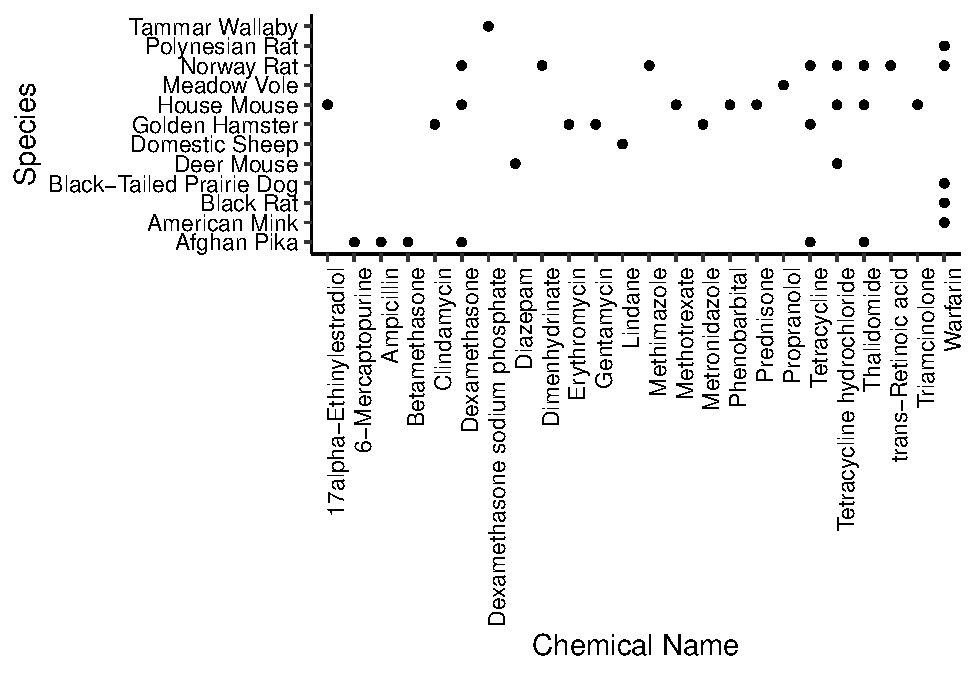
\includegraphics{Untitled_files/figure-latex/Exploratory 1-1.pdf}

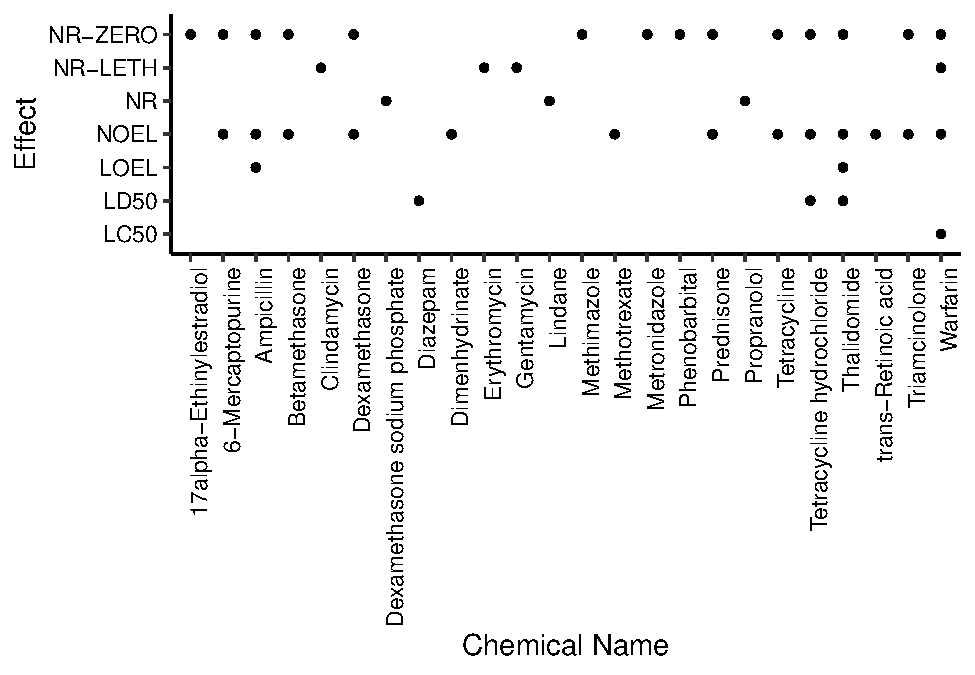
\includegraphics{Untitled_files/figure-latex/Exploratory 2-1.pdf}

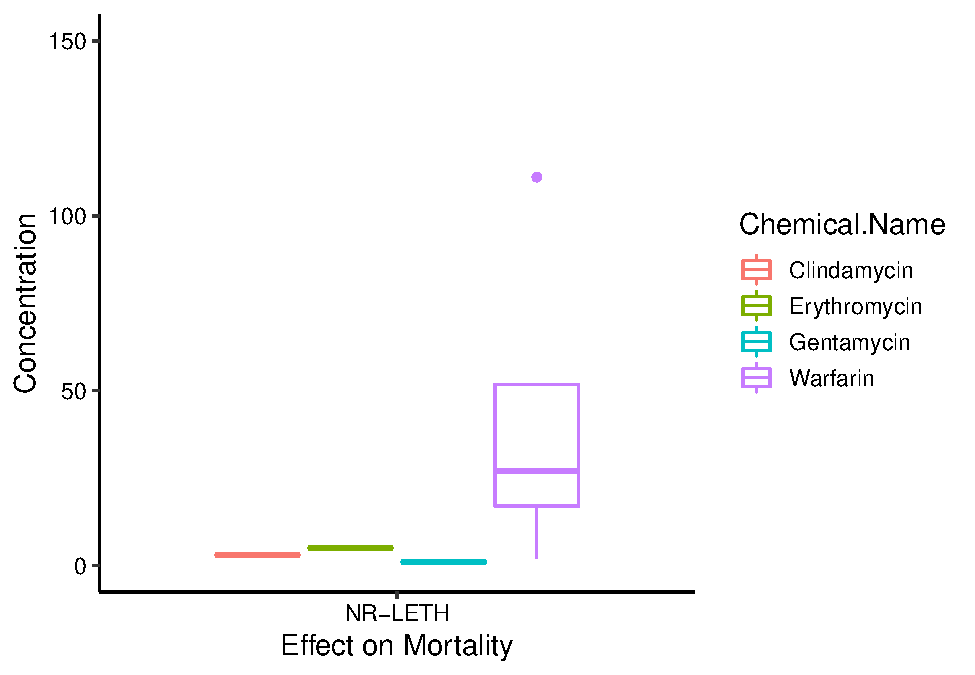
\includegraphics{Untitled_files/figure-latex/exploratory 3-1.pdf}

The first exploratory graph shows which drugs were tested on which
animals. This helps visualize if each drug was tested on each animal,
which could effect the results of cetain statistical tests. For the
second exploratory figure, I wanted to see which drugs resulted in which
endpoints. I was particulary interested to see which drugs resulted in
100\% mortality (NR-LETH). For the third exploratory figure, I
determined the spread of concentration for the drugs that caused 100\%
mortality (NR-LETH). I wanted to determine if certain drugs required
higher concentrations to kill and if certain drugs killed at multiple
concentrations.

\newpage

\section{Analysis}\label{analysis}

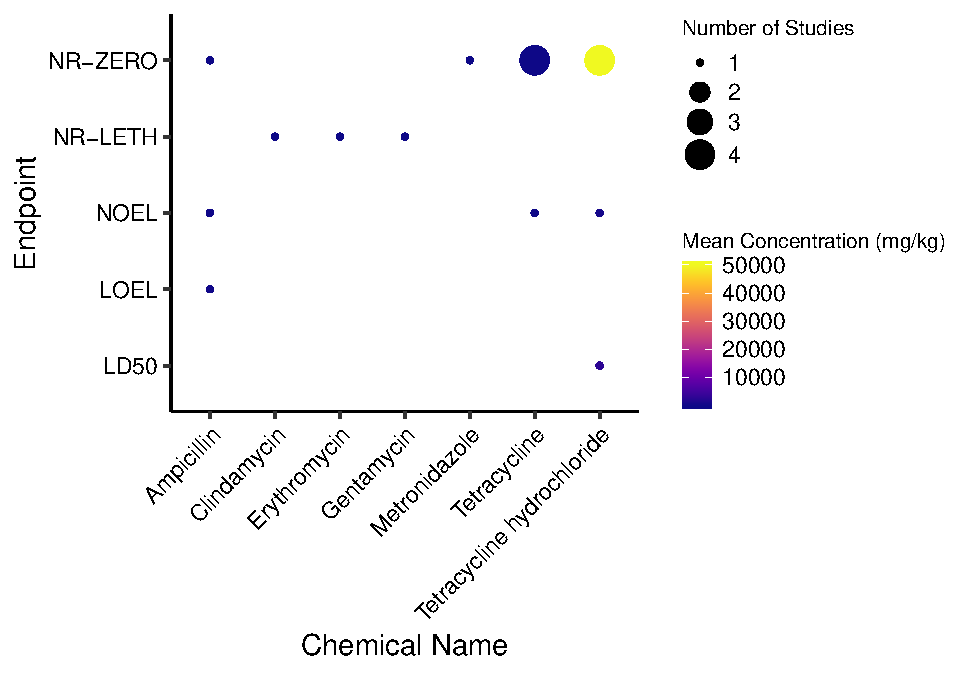
\includegraphics{Untitled_files/figure-latex/visualization 1-1.pdf}

\begin{verbatim}
## Warning: Ignoring unknown parameters: breaks
\end{verbatim}

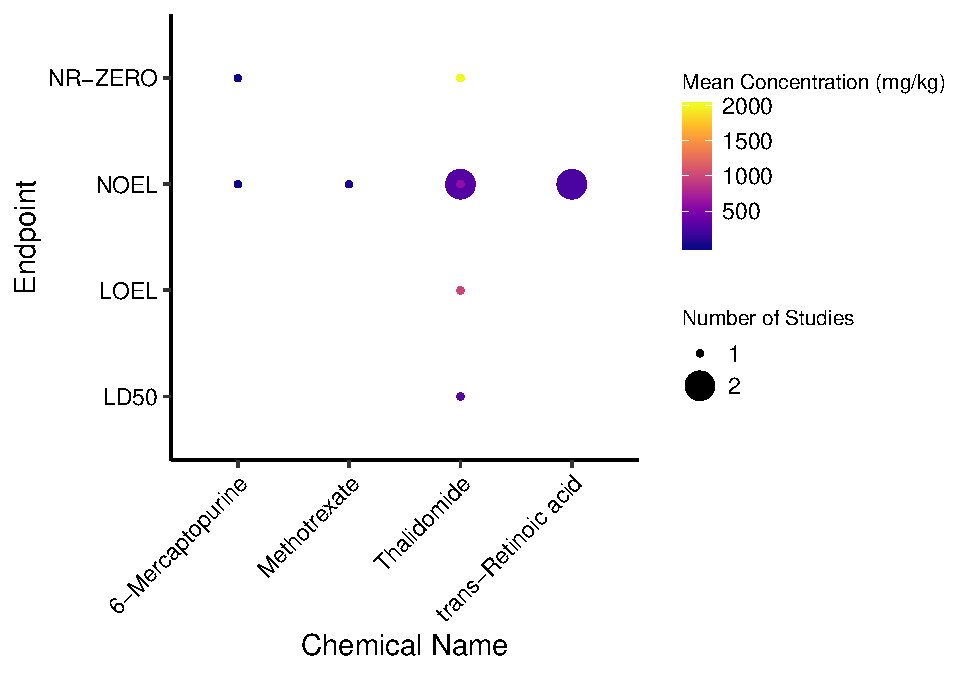
\includegraphics{Untitled_files/figure-latex/visualization 2-1.pdf}

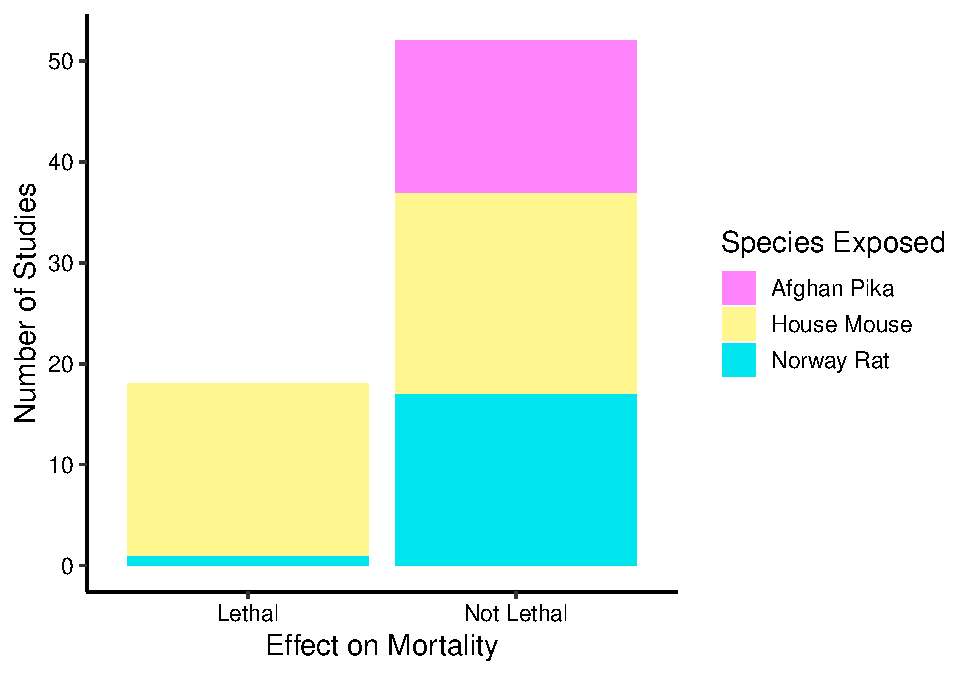
\includegraphics{Untitled_files/figure-latex/Visualization3-1.pdf}

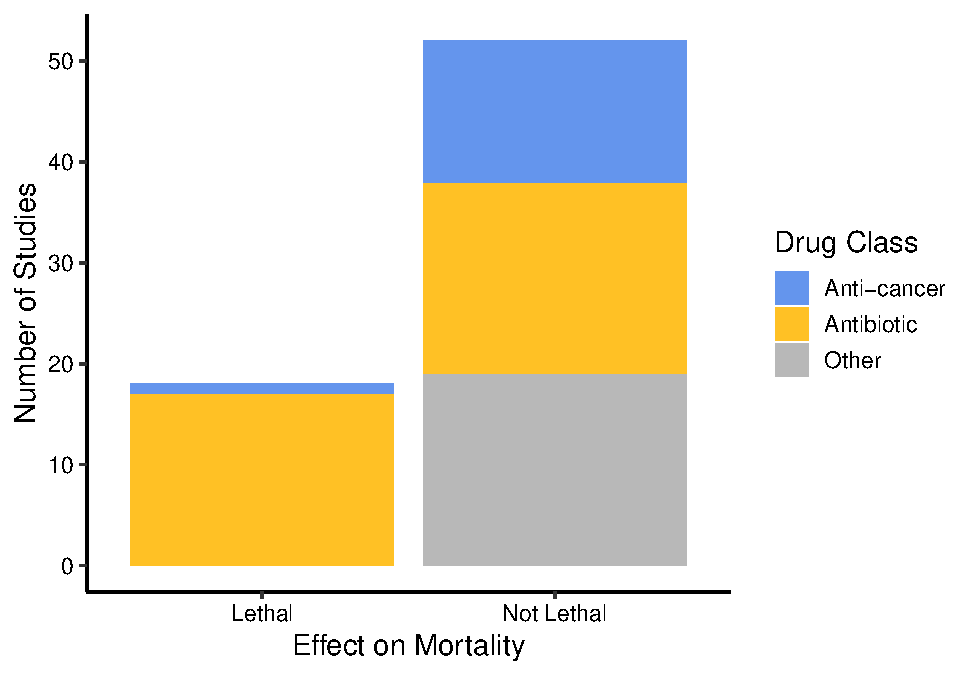
\includegraphics{Untitled_files/figure-latex/visualization4-1.pdf}

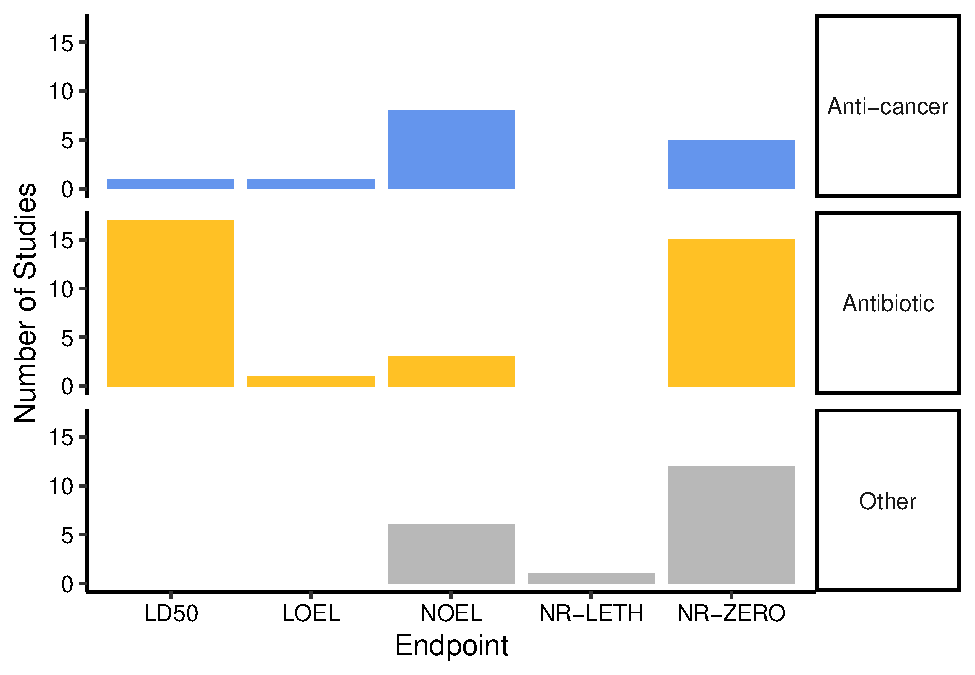
\includegraphics{Untitled_files/figure-latex/visualization5-1.pdf}

\newpage

\section{Summary and Conclusions}\label{summary-and-conclusions}


\end{document}
